\documentclass[a4paper, 10pt, twocolumn]{scrartcl}

% Vorlage fuer Poster
% Getestet mit pdfTeX; Kodierung: UTF8
% Version 2024-02-23

% Hier Titel, Name und Modul eintragen:
\newcommand{\thema}{Logistische Regression} % bei mehrzeiligem Thema \posterHeadHeight erhöhen
\newcommand{\name}{Thomas Sine-Nomine}
\newcommand{\modul}{Machine Learning}

\newcommand{\posterHeadHeight}{29mm}

% Einträge für das Literaturverzeichnis:
\begin{filecontents}[force]{literatur.bib}
@book{geron,
  title         = {Praxiseinstieg Machine Learning mit Scikit-Learn, Keras und TensorFlow},
  subtitle      = {Konzepte, Tools und Techniken für intelligente Systeme},
  author        = {Géron, Aurélien and Rother, Kristian and Demmig, Thomas},
  publisher     = {O'Reilly},
  location      = {Heidelberg},
  year          = {2020},
  edition       = {2},
}

@misc{logreg_wiki,
  title         = {Logistic regression},
  author        = {Wikipedia},
  url           = {https://en.wikipedia.org/w/index.php?title=Logistic_regression&oldid=1210273561},
  urldate       = {2024-02-26},
}

@online{logreg_basecamp,
  author        = {Data Basecamp},
  title         = {Was ist eine Logistische Regression?},
  year          = {2022},
  url           = {https://databasecamp.de/ki/logistische-regression},
  urldate       = {2024-02-26},
}
\end{filecontents}

\usepackage[style=numeric, backend=biber, bibencoding=utf8]{biblatex}
\usepackage{poster}
\newcommand{\spacer}{\vfill}

\begin{document}
% ============================== Block ==============================
\begin{block}{Überblick}
Die logistische Regression wird häufig zum Abschätzen der Wahrscheinlichkeit eingesetzt, dass ein Datenpunkt einer bestimmten Kategorie angehört (z.\,B.: Wie hoch ist die Wahrscheinlichkeit, dass eine E-Mail Spam enthält?). Wenn die geschätzte Wahrscheinlichkeit mehr als 50~\% beträgt, sagt das Modell vorher, dass der Datenpunkt zu dieser Kategorie gehört.

Somit lässt sich die logistische Regression im Gegensatz zu anderen Regressionsmodellen zur Klassifikation einsetzen.
\end{block}

\spacer

% ============================== Block ==============================
\begin{block}{Modellfunktion}
Als Modellfunktion kommt die Sigmoid"=Funktion zum Einsatz:

\begin{equation*}
h_{\theta}(x) = \frac{1}{1 + e^{-z}} \mathrm{~mit~} z = \theta^{T}x
\end{equation*}

Es handelt sich hierbei um eine nicht"=lineare Funktion. Die folgende Abbildung zeigt den Funktionsgraphen.

\begin{center}
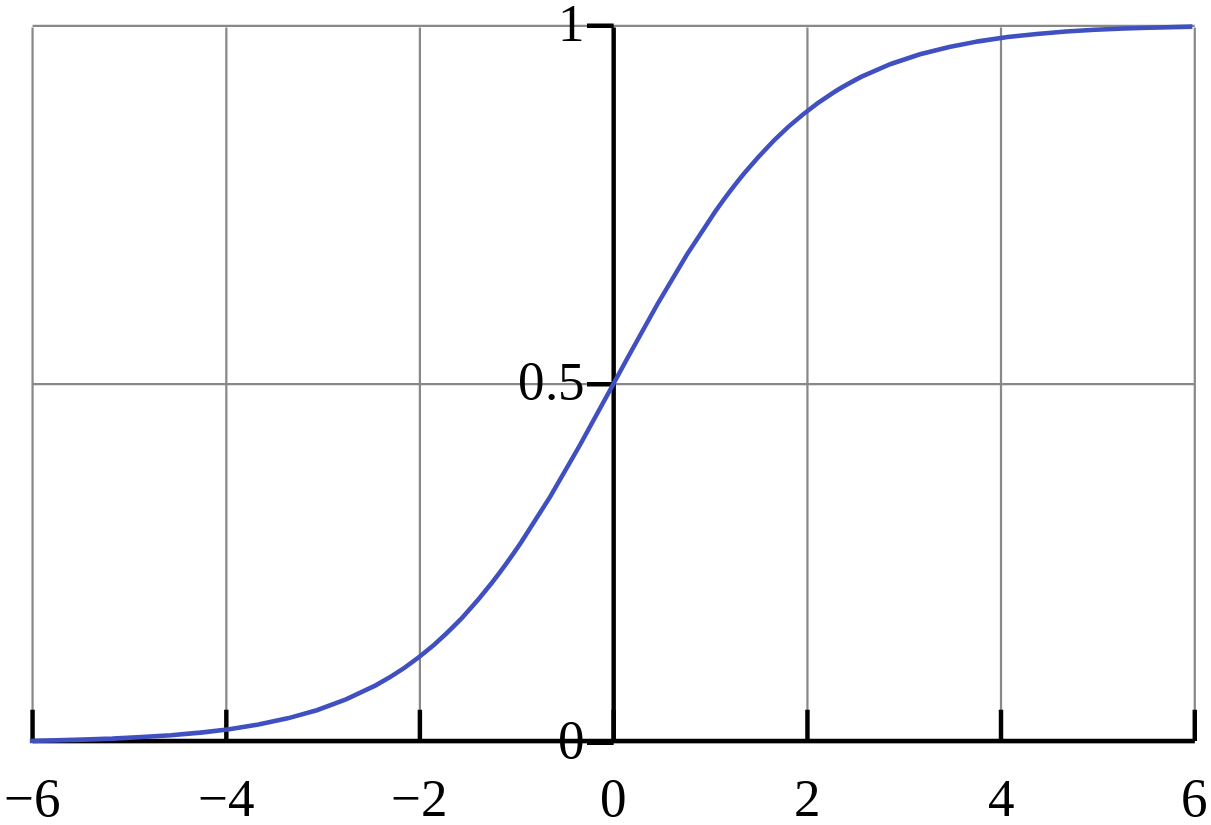
\includegraphics[width=0.5\linewidth]{logistisch_funkt}
\captionof{figure}{Logistische Funktion}%\label{beispielbild}
\end{center}
\end{block}

\spacer

% ============================== Block ==============================
\begin{block}{Kostenfunktion}
Für die Kostenfunktion wird die mittlere quadratische Abweichung (englisch \emph{mean squared error}) verwendet:

\begin{equation*}
\mathrm{MSE}(\theta) = \frac{1}{m} \sum_{i=1}^{m}(h_{\theta}(x^{(i)}) - y^{(i)})^{2} 
\end{equation*}

$\mathrm{MSE}(\theta)$ ist nicht konvex und besitzt in der Regel lokale Minima. Das Gradientenverfahren lässt sich auf diese Funktion nicht anwenden.
\end{block}

\spacer

% ============================== Block ==============================
\begin{block}{Anwendungsgebiete}
\begin{itemize}
\item Vorhersage von Wahlergebnissen
\item medizinische Diagnosen
\item Kaufverhalten
\item Prüfung von Kreditanträgen auf Risiken
\item Nutzerverhalten im Internet
\end{itemize}
\end{block}

% \spacer

% ============================== Block ==============================
\begin{block}{Beispiel-Usecase}
Eine Anwendungsmöglichkeit ist die Vorhersage des Bestehens bzw. Nicht"=Bestehens einer Prüfung in Abhängigkeit von der investierten Vorbereitungszeit.

\begin{center}
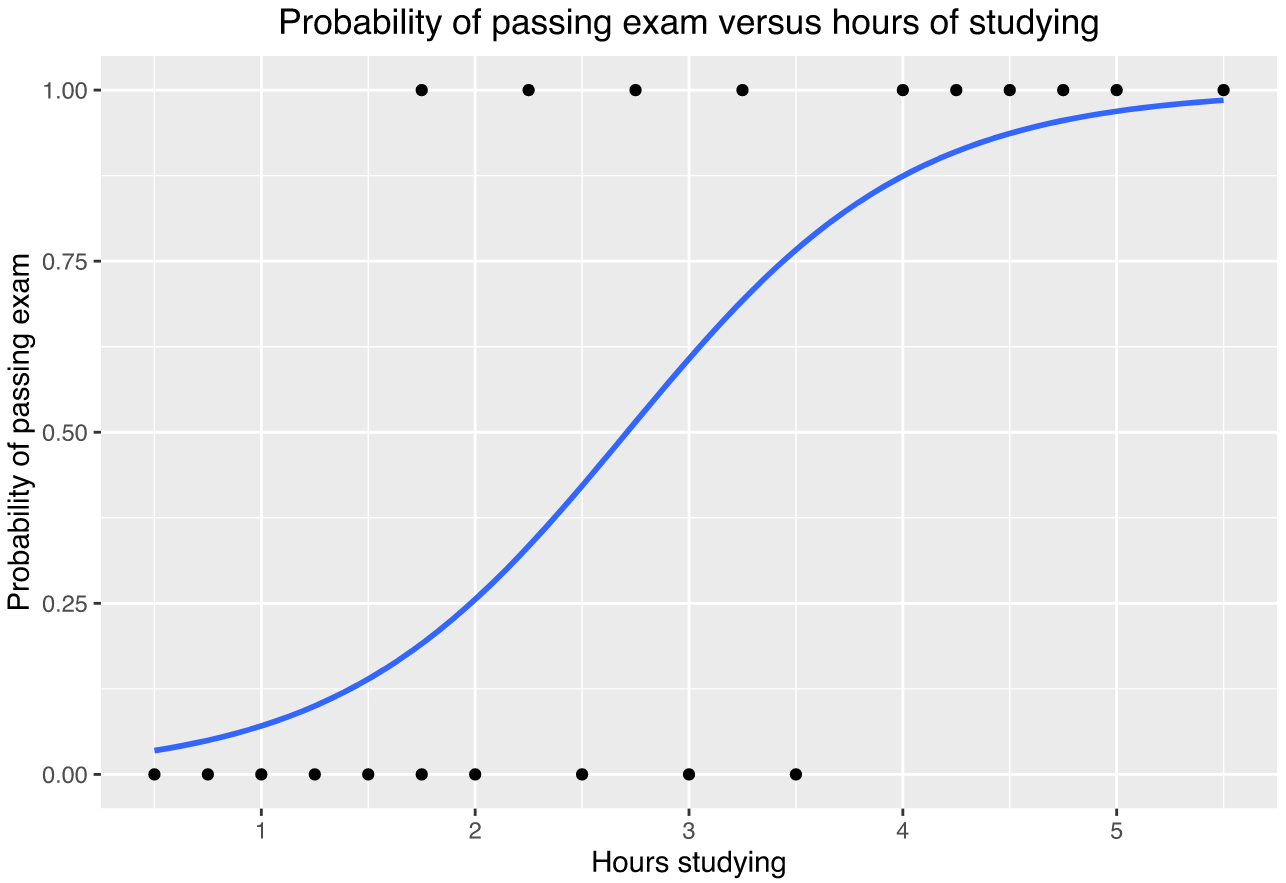
\includegraphics[width=1.0\linewidth]{logistisch_bsp}
\captionof{figure}{Vorhersage von Prüfungsergebnissen mittels logistischer Regression.}%\label{beispielbild}
\end{center}

Bei einem Funktionswert von $> 0,5$ ist ein Bestehen der Prüfung wahrscheinlicher.
\end{block}

\spacer

% ============================== Block ==============================
\begin{block}{Programmbeispiel}
In scikit"=learn ist die logistische Regression im Modul \lstinline{LogisticRegression} verfügbar. Das Training erfolgt wie gewohnt mit \lstinline{fit()}.

\begin{lstlisting}
from sklearn.linear_model import LogisticRegression
log_reg = LogisticRegression()
log_reg.fit(X, y)
\end{lstlisting}

Vorhersagen werden mittels \lstinline{predict} gemacht:

\begin{lstlisting}
log_reg.predict([[1.7], [1.5]])
\end{lstlisting}
\end{block}

\spacer

% ----- ab hier nichts mehr ändern -----
\nocite{*} % alle Quellen zeigen, auch wenn im Text nicht referenziert
\begin{block}{Literatur}
\printbibliography[heading=none]
\end{block}

\spacer
\end{document}
